% IEEE BigData Cup 2026, Challenge 02: 4-page technical report (IEEEtran conference template).
% Build: latexmk -pdf main.tex   (figures are in figures/; the folder can be uploaded to Overleaf as is)
\documentclass[conference]{IEEEtran}
\IEEEoverridecommandlockouts
\usepackage{cite}
\usepackage{amsmath,amssymb}
\usepackage{graphicx}
\usepackage{booktabs}
\usepackage{xcolor}
\usepackage{tikz}
\usetikzlibrary{arrows.meta,positioning}
\usepackage[hidelinks]{hyperref}
\usepackage{microtype}

\begin{document}

\title{Training for Panoptic Quality: Solar Filament\\ Segmentation at the Visibility Limit}

% TODO before submission: authors, affiliations, e-mail, and the repository URL in Section VII.
\author{\IEEEauthorblockN{Author Name(s)}
\IEEEauthorblockA{Affiliation, City, Country\\
e-mail}}

\maketitle

\begin{abstract}
Solar filaments are cool plasma held in the corona above magnetic polarity inversion lines (PILs), seen in
H$\alpha$ as thin, dark absorption features. We segment every filament in $2048\times2048$ GONG H$\alpha$ images
as a separate instance, scored by Panoptic Quality (PQ) against each of up to three annotators. A single
query-based model reads the whole disk through a FlashInternImage-L backbone. At native resolution it also reads
three physical channels, among them the cloud-model contrast $I/B-1$. The model is trained directly on a
differentiable PQ surrogate, with Noisy-Student self-training on 9,272 archive frames. It reaches PQ 0.40 on the
public leaderboard and 0.446 on held-out data, where two annotators agree at only 0.340. The labels explain this
ceiling. Annotator agreement falls from 0.79 to 0.25 as the filament contrast approaches the quiet-Sun texture,
and the model's misses follow the same visibility curve. The model also agrees with the annotators (PQ 0.43)
better than they agree with each other (0.33). Magnetograms show that the detections no annotator drew lie on
PILs as often as annotated filaments do.
\end{abstract}

\begin{IEEEkeywords}
solar filaments, H$\alpha$, cloud model, instance segmentation, panoptic quality, self-training, annotator agreement
\end{IEEEkeywords}

% Fig. 1: architecture of final-A (full text width). Thumbnails: paper/make_thumbnails.py.
\begin{figure*}[t]
\centering
\begin{tikzpicture}[x=0.975cm, y=0.92cm,
  arch/.style={draw=black!65, rounded corners=1pt, align=center, inner sep=1.1pt,
               font=\fontsize{5.5}{6.3}\selectfont},
  ctx/.style={arch, fill=blue!9}, det/.style={arch, fill=orange!13}, dec/.style={arch, fill=green!10},
  res/.style={arch, fill=gray!12}, train/.style={arch, dashed, fill=red!5},
  lab/.style={font=\fontsize{5.3}{6.1}\selectfont, align=center, inner sep=0.5pt},
  flow/.style={-{Stealth[length=1.1mm, width=0.9mm]}, draw=black!70, line width=0.45pt},
  line/.style={draw=black!70, line width=0.45pt}]
% ---------------- input
\node[inner sep=0] (img) at (0.88,3.2) {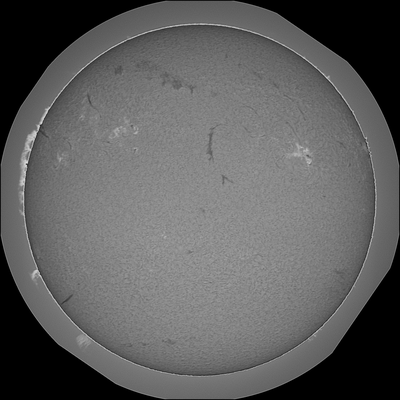
\includegraphics[width=1.66cm]{figures/arch_input.png}};
\node[lab, below=0.5mm of img] {H$\alpha$ image\\2048\textsuperscript{2} px (the\\only inference input)};
\coordinate (split) at (1.98,3.2);
\draw[line] (img.east) -- (split);
% ---------------- context branch
\node[lab, anchor=west] at (2.2,6.16) {\textbf{context branch}: FlashInternImage-L (DCNv4, 219\,M, ImageNet-22k$\to$1k);
  strides relative to 2048\,px};
\node[ctx, text width=0.8cm, minimum height=0.8cm] (rs) at (2.72,5.1) {resize to\\1024\textsuperscript{2}};
\node[ctx, text width=0.82cm, minimum height=1.45cm] (s1) at (3.86,5.1) {S1\\5 blocks\\160 ch\\/8};
\node[ctx, text width=0.82cm, minimum height=1.28cm] (s2) at (4.92,5.1) {S2\\5 blocks\\320 ch\\/16};
\node[ctx, text width=1.0cm, minimum height=1.11cm] (s3) at (6.08,5.1) {S3\\22 blocks\\640 ch\\/32};
\node[ctx, text width=0.82cm, minimum height=0.94cm] (s4) at (7.24,5.1) {S4\\5 blocks\\1280 ch\\/64};
\node[ctx, text width=0.82cm, minimum height=1.45cm] (fpn) at (8.36,5.1) {FPN\\$P_1$--$P_4$\\192 ch\\/8 to /64};
\draw[flow] (split) |- (rs.west);
\foreach \a/\b in {rs/s1, s1/s2, s2/s3, s3/s4, s4/fpn} \draw[flow] (\a) -- (\b);
% ---------------- native detail branch
\node[lab] at (3.7,2.42) {\textbf{native branch}, 2048\textsuperscript{2} px};
\node[inner sep=0] (c1) at (2.72,1.62) {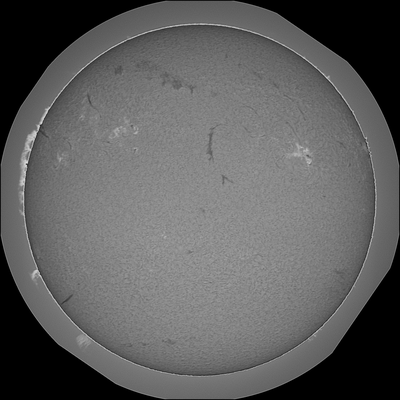
\includegraphics[width=0.84cm]{figures/arch_input.png}};
\node[inner sep=0] (c2) at (3.7,1.62) {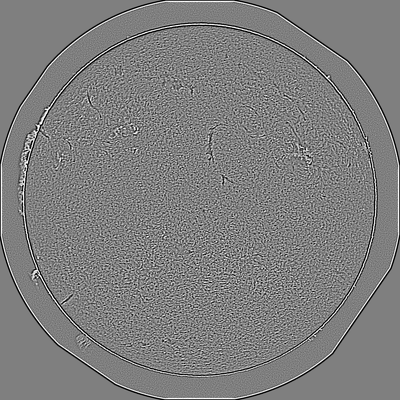
\includegraphics[width=0.84cm]{figures/arch_contrast.png}};
\node[inner sep=0] (c3) at (4.68,1.62) {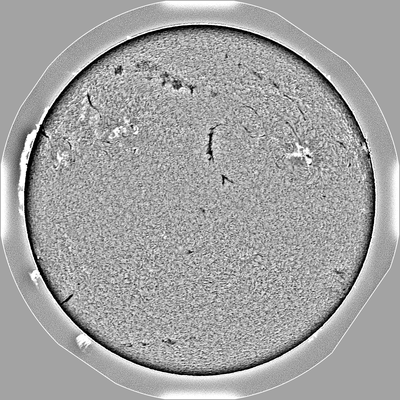
\includegraphics[width=0.84cm]{figures/arch_darkness.png}};
\node[lab, below=0.4mm of c1] {intensity\\$I$};
\node[lab, below=0.4mm of c2] {local\\contrast};
\node[lab, below=0.4mm of c3] {darkness\\$I/B-1$};
\draw[flow] (split) |- (c1.west);
\node[det, text width=0.95cm, minimum height=1.15cm] (h1) at (5.88,1.62) {Haar 2$\times$2\\(4 phases)\\1$\times$1 conv\\32 ch, /2};
\node[det, text width=1.1cm, minimum height=1.15cm] (g2) at (7.05,1.62) {gate $\oplus P_1$\\curve block\\32 ch, /2};
\node[det, text width=1.1cm, minimum height=1.15cm] (g4) at (8.3,1.62) {Haar\\gate $\oplus P_1$\\curve block\\64 ch, /4};
\draw[flow] (c3.east) -- (h1.west);
\draw[flow] (h1) -- (g2);
\draw[flow] (g2) -- (g4);
\draw[line] (fpn.south) -- ++(0,-1.15) coordinate (pdown);
\draw[flow] (pdown) -| (g2.north);
\draw[flow] (pdown) -| (g4.north);
\node[lab, anchor=west] at (8.4,3.4) {$P_1$};
\node[lab, text=black!65] at (7.0,0.72) {\itshape at inference in 512\,px tiles with a 48\,px halo};
\node[det, text width=1.22cm, minimum height=0.46cm] (f4) at (9.76,2.22) {$F_4$: 192 ch, /4};
\node[det, text width=1.22cm, minimum height=0.46cm] (m2) at (9.76,1.62) {$M_2$: 64 ch, /2};
\node[det, text width=1.22cm, minimum height=0.46cm] (ph) at (9.76,1.02) {$\Phi_2$: 32 ch, /2};
\draw[flow] (g4.east) -- (f4.west);
\draw[flow] (g4.east) -- (m2.west);
\draw[flow] (m2) -- (ph);
% ---------------- query decoder
\node[dec, text width=3.5cm, minimum height=0.86cm] (mem) at (12.62,5.1)
  {\textbf{scene memory}: $F_4$, $P_2$, $P_3$ average-pooled to 48\textsuperscript{2}, 24\textsuperscript{2},
   12\textsuperscript{2} cells, plus 256 unpooled $F_4$ tokens at seed-map peaks};
\node[dec, text width=1.0cm, minimum height=0.62cm] (seed) at (11.48,3.82) {seed map\\(skeleton)};
\node[dec, text width=1.0cm, minimum height=0.85cm] (qi) at (11.48,2.92) {64 queries\\at diverse\\seed peaks};
\node[dec, text width=1.9cm, minimum height=2.9cm, align=left] (layer) at (13.36,3.0)
  {\textbf{6 decoder layers}\\[1.2pt]
   $\cdot$ self-attention\\
   $\cdot$ cross-attention to the memory, masked by the query's own mask (global every 2nd layer)\\
   $\cdot$ attention to 64 native points of its mask (32 foreground, 32 edge)\\
   $\cdot$ FFN, mask feedback};
\node[train, text width=2.05cm, minimum height=0.5cm] (pilot) at (13.36,0.8) {+32 mask pilots from noised GT masks (training only)};
\draw[flow] (fpn.east) -- node[lab, above] {$P_2,P_3$} (mem.west);
\draw[line] (f4.east) -- ++(0.24,0) coordinate (bus);
\draw[flow] (bus) |- ([yshift=-2.6mm]mem.west);
\draw[flow] (bus |- seed.west) -- (seed.west);
\draw[flow] (bus) |- ([yshift=-11mm]layer.west) node[lab, above, pos=0.78] {native points};
\draw[flow] (seed) -- (qi);
\draw[flow] (qi.east) -- (qi.east -| layer.west);
\draw[flow] (layer.north |- mem.south) -- (layer.north);
\draw[flow, dashed] (pilot) -- (layer);
% ---------------- heads, native rendering, test-time augmentation
\node[res, text width=1.25cm, minimum height=1.45cm] (head) at (15.22,4.32)
  {per query\\$P(\text{filament})$\\quality $\approx$ IoU\\$e\in\mathbb{R}^{64}$\\$\varphi\in\mathbb{R}^{8}$};
\node[res, text width=1.32cm, minimum height=1.55cm] (rend) at (15.22,2.3)
  {native logits\\$\uparrow_2(e^{\top}\!M_2)$\\$+\,\mathrm{PS}(\varphi^{\top}\Phi_2)$\\$\to$ 2048\textsuperscript{2} px};
\draw[flow] (layer.east |- head.west) -- (head.west);
\draw[flow] (head) -- (rend);
\draw[line] (m2.east) -- ++(0.12,0) coordinate (mbus);
\draw[line] (mbus) -- (mbus |- 0,0.3) coordinate (low);
\draw[line] (ph.south) -- (ph.south |- low);
\draw[flow] (ph.south |- low) -| (rend.south);
\node[res, text width=1.52cm, minimum height=1.5cm] (tta) at (17.1,4.55)
  {$\times$8 dihedral views\\cluster (IoU$>$0.5),\\average; keep\\score $\ge$ 0.10,\\mask $p\ge$ 0.40;\\pixel ownership};
\node[inner sep=0] (out) at (17.1,2.26) {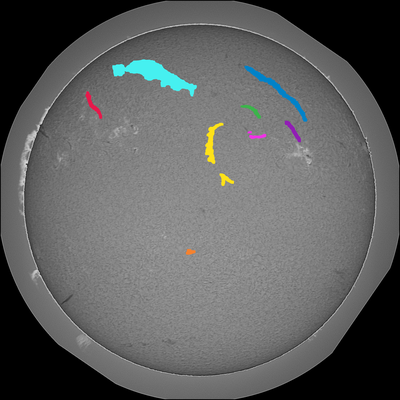
\includegraphics[width=1.55cm]{figures/arch_output.png}};
\node[lab, below=0.5mm of out] {non-overlapping\\instances};
\draw[flow] (rend.east) -- ++(0.22,0) |- (tta.west);
\draw[flow] (tta) -- (out);
% ---------------- training objective
\node[train, text width=5.7cm] (loss) at (14.98,6.12)
  {\textbf{training}: Hungarian matching per annotator record, $-\log\widetilde{\mathrm{PQ}}$ on 16,384 native
   points, auxiliary losses $\times$0.02};
\end{tikzpicture}
\Description{Block diagram: an H-alpha image feeds a context branch (resize, FlashInternImage-L stages, FPN) and a native
branch (intensity, local contrast and darkness channels, Haar split, gated curve blocks); both feed a query decoder whose
per-query heads render native-resolution masks, fused over eight dihedral views into non-overlapping instances.}
\caption{Architecture of final-A (223.6\,M parameters, 97.9\,\% in the backbone) at inference on a test
observation. A pretrained backbone sees the whole disk at 1024\,px, and a native branch reads three physical
channels at 2048\,px. Queries start at peaks of a skeleton-like seed map and render full-resolution masks from a
stride-2 basis $M_2$ plus a pixel-shuffled ($\mathrm{PS}$) phase term. Dashed boxes are training-only.}
\label{fig:pipeline}
\end{figure*}


\section{Introduction}
Filaments are prominences seen against the solar disk. They are plasma about a hundred times cooler and denser
than the surrounding corona, held tens of megametres above the photosphere in magnetic dips along PILs of the
photospheric field~\cite{martin1998filaments,mackay2010prominences}. In the core of H$\alpha$ they absorb and
scatter the chromospheric radiation from below and appear dark. Beyond the limb, the same plasma shines as a
prominence. An erupting filament can launch a coronal mass ejection, so catalogues of individual filaments are a
standing input to space-weather research~\cite{ahmadzadeh2019filament,diercke2024filaments}.

The IEEE BigData Cup 2026 filament challenge~\cite{bigdatacup2026} asks for every filament in a
GONG~\cite{harvey1996gong} H$\alpha$ full-disk image as a separate instance, and it scores PQ~\cite{kirillov2019panoptic}
against each annotator's drawing. Three properties of the observations shape the problem. At about 0.74\,Mm per
pixel, filaments are only 6--10\,Mm wide (median inscribed width 14\,px, 10\,\% at most 8\,px) but up to
400\,Mm long. Many are faint: a filament is only as visible as its absorption against the mottled chromosphere
around it. And the labels inherit this, since two annotators of the same image agree at PQ 0.340.

We contribute three things:
(i)~a single query-based instance segmenter that keeps native resolution, reads a physically normalized contrast
channel and is trained end to end on a differentiable PQ surrogate;
(ii)~Noisy-Student self-training~\cite{xie2020noisystudent} on unlabelled archive frames, where teacher
diversity mattered more than pool size;
(iii)~an observation-physics analysis of the labels. Annotator agreement and model misses follow the same
visibility curve in the cloud-model contrast, the model agrees with the annotators better than they agree with
each other, and its unlabelled detections are as magnetically plausible as annotated filaments.

\section{Data and Metric}
MAGFiLO~\cite{ahmadzadeh2024magfilo} provides 707 training observations from the six GONG sites (2011--2022) with
1,154 annotator records. Of these observations, 411 were drawn once, 145 twice and 151 three times, for 8,199
filament polygons (median area 1,228\,px). The test set has 180 observations. PQ is computed for every annotator
record and then pooled. A pair with IoU\,$>$\,0.5 is a true positive, and
$\mathrm{PQ}=\sum_{\mathrm{TP}}\mathrm{IoU}/(|\mathrm{TP}|+\frac12|\mathrm{FP}|+\frac12|\mathrm{FN}|)$. One set of
predictions is therefore scored against every annotator's version of an observation, and no single answer can
match all of them. We split the observations into five folds by a hash of the file name and selected models on
fold~0 (120 observations, 192 records, 1,341 filaments).

\emph{Compliance.} Inference reads only the provided H$\alpha$ test image. Training uses the competition polygons
and our own pseudo-labels. It uses no annotator identities or other ground-truth metadata, and no archive frame
from a test-image day.

\section{Method}
\subsection{Physically normalized inputs}
A pretrained backbone needs the whole disk to tell filaments from sunspots, plage and the limb, while the outline
needs native pixels. The model therefore reads the image twice (Fig.~\ref{fig:pipeline}): as a 1024\,px context
view, and as three native 2048\,px channels. Two of them are the intensity $I$ and a local contrast
$4(I-\bar I_{15\times15})$. The third encodes the absorption physics. In Beckers' cloud
model~\cite{beckers1964cloud}, a filament of optical depth $\tau$ and source function $S$ in front of a background
of intensity $I_0$ is observed at $I=I_0e^{-\tau}+S(1-e^{-\tau})$. Its relative contrast is
\begin{equation}
C=\frac{I}{I_0}-1=\Big(\frac{S}{I_0}-1\Big)\big(1-e^{-\tau}\big).
\label{eq:cloud}
\end{equation}
$C$ grows with $\tau$ for optically thin filaments and saturates at $S/I_0-1$ for thick ones. Dividing by the
background removes exposure, sky transparency and the centre-to-limb darkening of $I_0$, which change $I$ by
large factors within and between frames. What remains is set by the filament's $\tau$ and its $S/I_0$. We
estimate $I_0$ by the quiet-Sun background $B$: a normalized convolution over the disk only, with
$\sigma\approx32$\,px, wider than any filament, so that the dark sky never biases $B$ at the limb. The model is
fed $4(I/B-1)$, set to zero off the disk.

\subsection{Architecture}
\emph{Context branch.} FlashInternImage-L~\cite{xiong2024dcnv4} (DCNv4, ImageNet-22k$\to$1k) gives a four-level
pyramid, fused FPN-style to 192 channels.
\emph{Native branch.} An orthogonal $2\times2$ Haar split~\cite{xu2023haar} keeps all four sub-pixel phases of the
native channels, three of which a strided convolution would discard, so the edges of a 6--10\,Mm filament stay
resolved to a pixel. Gated context features follow, and then \emph{curve blocks}, which aggregate features along
two continuously bending 7-point curves after dynamic snake convolution~\cite{qi2023dsconv}, because filament
spines bend.
\emph{Query decoder.} As in Mask2Former~\cite{cheng2022mask2former}, 64 queries pass through 6 layers of
self-attention, cross-attention restricted to their current mask, and a feed-forward network. Every second
layer attends globally, so a missed branch can be recovered. A seed map, trained to predict filament skeletons,
supplies the queries' starting points: 64 spatially diverse peaks, so that one long filament cannot attract
all the queries. It also supplies 256 unpooled memory tokens. Together with 64 native points that each query
reads on its own mask, these tokens keep an 8\,px filament from being averaged away in the pooled memory. Each
query predicts $P(\text{filament})$, a quality (its native IoU) and an embedding that renders its mask at
2048\,px from a stride-2 basis plus a sub-pixel phase term. During training, 32 mask-pilot
queries~\cite{zhang2023mpformer} reconstruct noised ground-truth masks.

\subsection{Training on Panoptic Quality}
The Hungarian algorithm~\cite{carion2020detr} matches each annotator record to the queries. The main loss is
$-\log\widetilde{\mathrm{PQ}}$, a differentiable PQ over the batch, evaluated on 16,384 importance-sampled native
pixels per image. With query confidence $c_q=P_q(\text{filament})\,\sigma(\text{quality}_q)\,\bar p_q$,
\begin{equation}
\widetilde{\mathrm{PQ}}=\frac{\sum_q d_q\,t_q\,\mathrm{IoU}_q}{\frac12\sum_q d_q+\frac12|G|},
\end{equation}
where $d_q=\sigma((c_q-0.15)/0.05)$ is a soft detection, $t_q=\sigma((\mathrm{IoU}_q-0.5)/0.1)$ a soft true
positive and $|G|$ the number of drawn filaments. $\mathrm{IoU}_q$ is measured on the pixels that query $q$ owns
under a per-pixel softmax of $(\log\sigma(\ell_q)+\log c_q+\log d_q)/0.15$ over the queries, which mirrors the
pixel competition at inference. The loss follows MaX-DeepLab~\cite{wang2021maxdeeplab}, but it scores native
masks under the inference rule. Auxiliary losses (weight 0.02) cover classification, point-sampled BCE and Dice,
the quality head, deep supervision and the seed map.

\subsection{Stages and Noisy-Student self-training}
Each training stage is warm-started from the previous one (Table~\ref{tab:stages}). Training on the PQ surrogate
raised the single-view fold-0 PQ from 0.169 to 0.395. The limb-flattened channel, together with arbitrary
rotation and scale augmentation, added 0.007. We then followed Noisy Student~\cite{xie2020noisystudent}.
Unlabelled GONG frames of the same instrument, from random days of 2011--2022, were labelled by two fold-0
teachers (views d0 and f2 of each, fused like a submission with mask threshold 0.70). Frames from test-image days
were never labelled. Each epoch mixed all labelled records with as many pseudo-labelled frames under strong
noise. Round~1 (teachers E3 and E6, 3,028 frames) produced F1. Round~2 (teachers E9 and E6, 9,272 frames from
3,465 days) produced the submitted model final-A, trained for 12 more epochs at a quarter of the learning rate. A
third round taught by final-A alone lowered the public score to 0.38: teacher diversity mattered more than pool
size.

\begin{table}[t]
\caption{Training stages: fold-0 PQ (single view) and public PQ (8 views).}
\label{tab:stages}
\centering
\begin{tabular}{@{}llcc@{}}
\toprule
Stage & Change & Fold 0 & Public\\
\midrule
S2 & S1 (0.169) + PQ surrogate as main loss & 0.348 & --\\
S3 & mask pilots, seeded queries & 0.375 & 0.33$^a$\\
v7 & soft surrogate, $-\log$ objective & 0.395 & 0.37\\
E3 & limb-flattened channel, rotations & 0.403 & --\\
E9 & E3 + round-1 pseudo-labels & 0.413$^b$ & --\\
F1 & E9 recipe on all labels & -- & 0.39\\
final-A & F1 + round-2 pseudo-labels & -- & \textbf{0.40}\\
\bottomrule
\end{tabular}\\[2pt]
{\footnotesize $^a$single view. $^b$optimistic: its pool held archive frames from fold-0 days.}
\end{table}

\subsection{Inference}
Each test image is segmented in its eight dihedral views (rotations by $k\cdot90^\circ$, with and without a
flip). These are exact pixel permutations that never interpolate a thin filament; a flip reverses chirality but
not the outline. The views' probability maps are mapped back, clustered by IoU\,$>$\,0.5 and averaged, and the
fused score is the summed member score divided by 8. Instances with score\,$\ge$\,0.10 are binarized at 0.40 and
claim pixels in score order, which yields non-overlapping masks. The threshold 0.40 is close to the IoU-optimal
$J/(1+J)$ for an attainable IoU $J\approx0.68$~\cite{nowozin2014iou}. All thresholds were chosen on fold~0.
Inference takes 3.7\,s per image on one RTX~3090.

\section{Results}
Because final-A (public PQ 0.40) has seen all labels, Table~\ref{tab:metrics} reports the organizers' judging
metrics for its fold-0 twin E9, the same recipe trained without the fold-0 labels. v7, trained without external
data, is the reference. Pair Dice and IoU average over all overlapping pairs, as in the organizers' notebook.
DiceScore is the \texttt{torchmetrics} Dice of the binary mask per record.

\begin{table}[t]
\caption{Judging metrics on held-out fold 0 (8 views, submission setting).}
\label{tab:metrics}
\centering
\setlength{\tabcolsep}{4.5pt}
\begin{tabular}{@{}lcc@{}}
\toprule
 & E9 (final recipe) & v7\\
\midrule
PQ (SQ / RQ) & \textbf{0.446} (0.678 / 0.658) & 0.436\\
TP / FP / FN & 810 / 311 / 531 & 790 / 320 / 551\\
Pair Dice / IoU, mean & \textbf{0.728} / 0.597 & 0.711 / 0.580\\
DiceScore per record (pooled) & 0.656 (0.684) & 0.660 (0.691)\\
GT overlapped by 0/1/2 pred. & 316 / 1001 / 24 & 306 / 1005 / 27\\
Pred.\ overlapping 0/1/2/3 GT & 131 / 935 / 51 / 4 & 122 / 917 / 62 / 9\\
\bottomrule
\end{tabular}
\end{table}

The instance structure is almost one-to-one. Of the ground-truth filaments that any prediction overlaps, 97.7\,\%
are overlapped by exactly one, and 94.4\,\% of the overlapping predictions overlap exactly one filament. Most
errors therefore concern whole filaments: 316 drawn filaments have no overlapping prediction (most of them
small), and 131 predictions overlap nothing drawn. Self-training raised PQ by 0.010 and pair Dice by 0.018 and reduced
merges from 71 to 55, while the pixel DiceScore stayed within 0.007. The gain is in instance correctness, not in
filament area.

\begin{figure}[t]
\centering
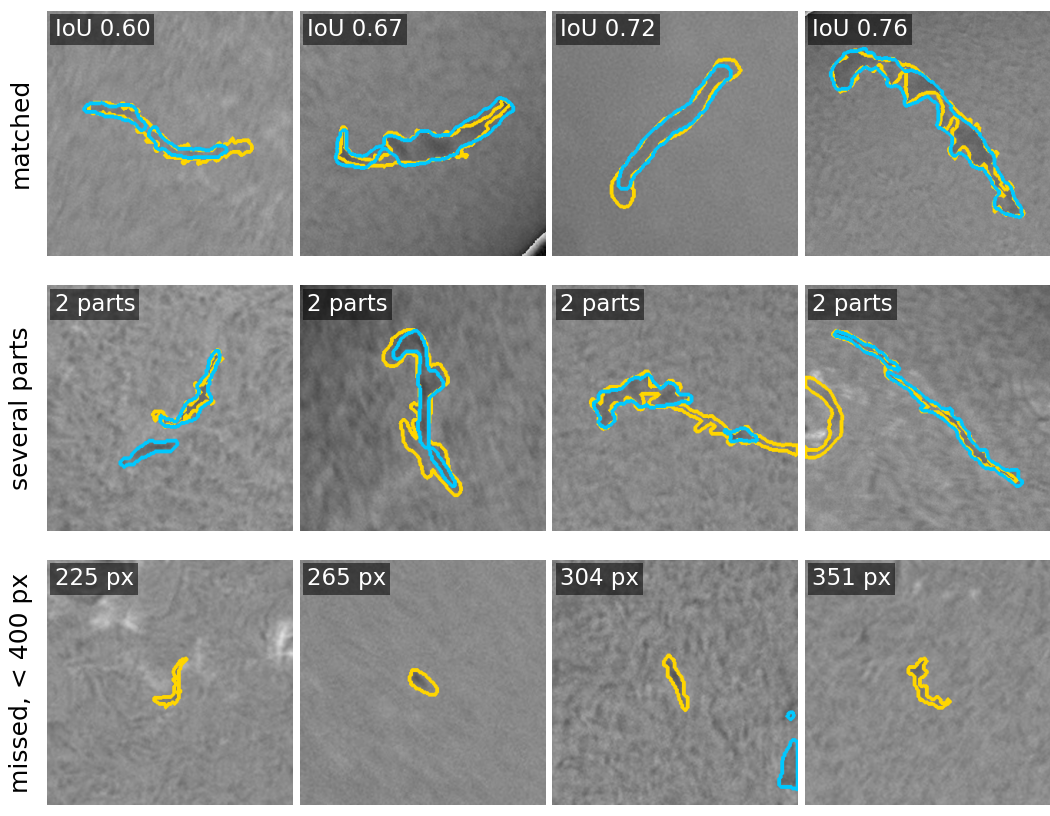
\includegraphics[width=0.88\columnwidth]{figures/morphology_details.png}
\caption{Fold-0 close-ups at fixed ranks, not hand-picked (annotator yellow, prediction cyan). Top: matched
filaments at the 20/40/60/80th IoU percentile. Middle: predictions in two parts. Bottom: missed filaments below
400\,px.}
\label{fig:morphology}
\end{figure}

\emph{Morphology} (Fig.~\ref{fig:morphology}). Predicted outlines follow the spines, their curvature and their
barbs at native resolution. They are slightly wider than the hand-drawn polygons (median inscribed width 16.8
vs.\ 14.4\,px) and more convex (solidity 0.67 vs.\ 0.58). Seeing blurs every edge over a few pixels, so where an
edge lies is partly a convention, and the 0.40 threshold deliberately favours generous outlines that match more
annotators. One prediction in five has several parts. The gap lies where the absorption along a filament channel
weakens, and there the annotator draws one continuous polygon: the model has learned the convention of one
instance per channel, not per connected dark region. The typical misses are compact, faint filaments of
200--400\,px. Test predictions have the shape statistics of the fold-0 predictions (median area 1,385 vs.\
1,296\,px), so there is no sign of a domain shift.

\section{The Visibility Limit of the Labels}
Why does the score saturate near the inter-annotator level? For each annotated filament we measured its mean
contrast $C$ (Eq.~\eqref{eq:cloud} with $I_0=B$), its area, its disk position $\mu=\cos\theta$, whether the
fold-0 model matched it, and its \emph{agreement}: the share of the other annotators of that observation who drew
it at IoU\,$>$\,0.5 (4,993 filaments on the 296 multi-record observations). To compare observations, we also
express $-C$ in units of the quiet-Sun texture $\sigma$, the robust per-pixel spread of $I/B-1$ that fibrils,
mottles and noise produce on the inner disk (median $\sigma=0.048$).

\begin{figure}[t]
\centering
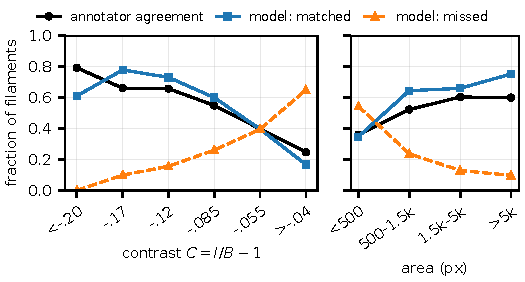
\includegraphics[width=\columnwidth]{figures/visibility.pdf}
\caption{Annotator agreement (the share of the other annotators who drew a filament) and the fold-0 model's match
and miss rates, against filament contrast $C$ (bin centres) and area.}
\label{fig:visibility}
\end{figure}

Agreement falls monotonically with contrast (Fig.~\ref{fig:visibility}), from 0.79 for the darkest filaments
($C<-0.20$) to 0.25 for the faintest ($C>-0.04$). In units of the texture it is 0.26 below $1\sigma$, 0.49 at
1--$2\sigma$ and 0.70 beyond $3\sigma$, and 58\,\% of all annotated filaments lie within $2\sigma$ of the texture.
Agreement also falls with size, from 0.60 above 1,500\,px to 0.36 below 500\,px. Size and contrast act
separately: fainter filaments are, if anything, larger (Spearman $\rho=0.29$), yet less often agreed on.
Agreement falls toward the limb as well (0.37 at $\mu<0.5$), although limb filaments are as dark as central ones
(median $C$ $-0.089$ vs.\ $-0.094$) and larger (1,846 vs.\ 1,116\,px). There the elevated filament is seen
obliquely, and its projected outline is ambiguous. The labels are thus visual detections near a contrast
threshold, not a complete census, and their completeness depends on the observing conditions as much as on the
Sun. The model's misses follow the same curve. It misses 0--10\,\% of the dark filaments without any overlap, but
65\,\% of the faintest bin. Its match rate equals or exceeds the human agreement everywhere except in the
darkest bin (18 filaments, extent errors) and below $1\sigma$ (0.15 vs.\ 0.26).

\begin{table}[t]
\caption{Model vs.\ annotators, scored the same way on the same 47 multi-record fold-0 observations: PQ at four
IoU thresholds, and the share of reference filaments matched, near-missed (best IoU 0.1--0.5) or absent.}
\label{tab:human}
\centering
\setlength{\tabcolsep}{3.5pt}
\begin{tabular}{@{}lccccccc@{}}
\toprule
 & \multicolumn{4}{c}{PQ at IoU $>$} & \multicolumn{3}{c}{reference filaments (\%)}\\
\cmidrule(lr){2-5}\cmidrule(l){6-8}
 & 0.3 & 0.4 & 0.5 & 0.6 & match & near & absent\\
\midrule
model vs.\ record & 0.483 & 0.468 & \textbf{0.430} & 0.347 & 60.0 & 15.9 & 24.1\\
record vs.\ record & 0.408 & 0.378 & 0.327 & 0.222 & 51.8 & 27.2 & 21.0\\
\bottomrule
\end{tabular}
\end{table}

In Table~\ref{tab:human}, the model agrees with the annotators better than they agree with each other at every
IoU threshold, and the gap widens as the threshold tightens. It near-misses far fewer reference filaments than a
second annotator (16 vs.\ 27\,\%), but it misses slightly more faint ones entirely (24 vs.\ 21\,\%).

\emph{A magnetic check.} Filaments form above PILs~\cite{martin1998filaments,mackay2010prominences}, which an
H$\alpha$ image cannot show. We paired every training observation with a line-of-sight magnetogram taken close in
time: 612 GONG 10-minute averages from the same site and 95 SDO/HMI~\cite{scherrer2012hmi} maps, 702 of the 707
within 15\,min. We smoothed $B_{\mathrm{LOS}}$ at 18.5\,Mm and marked PILs where the $\pm0.5$\,G regions touch.
Annotated filaments lie within 20\,Mm of a PIL 4.8 times as often as random disk points (23.3 vs.\ 4.9\,\%),
independent of their contrast or agreement. The share falls from 30\,\% at disk centre ($\mu\ge0.85$) to 12\,\%
near the limb ($\mu<0.6$), but random points fall alike (7.3 to 2.9\,\%), so the enrichment stays near 4. The
loss is therefore in the magnetograms: the line-of-sight component of the mostly vertical photospheric field
scales with $\mu$, and weak PILs drop below detection toward the limb. On fold~0, matched predictions (24\,\%),
predictions that no annotator drew (22\,\%) and missed filaments (23\,\%) cannot be told apart. The unlabelled
detections are thus as magnetically plausible as annotated filaments, and the misses are set by visibility rather
than by the magnetic configuration. The magnetograms serve this analysis only and are never used for training or
inference.

\section{What Did Not Work}
A change was adopted only if it gained 0.003 fold-0 PQ or improved the public score. We rejected the following:
discrete-PQ training (0.375$\to$0.322), curve-query and dynamic-mask decoders, multi-hypothesis decoding
($-0.004$), ensembles and multi-scale TTA (fold-0 PQ up to 0.452, public 0.38), weight averaging, arbitrary-angle
TTA, sharpness-aware and consistency fine-tuning (public 0.39), copy-paste of small filaments (public 0.38), and
post-processing ($\le$+0.002). An annotator-conditioned decoder (+0.002) was removed because annotator identities
are ground-truth metadata. The recall-oriented changes failed because they push detection into the regime where
annotators agree only 25--40\,\% of the time.

\section{Conclusion}
A single PQ-trained query model with a cloud-model contrast input, Noisy-Student self-training and dihedral TTA
reaches PQ 0.40 (public) and 0.446 (held out), above the 0.340 at which two annotators agree. Its remaining
errors are set by optical depth, seeing and the annotators' detection threshold rather than by model capacity.
Higher scores on this benchmark will therefore need labels that record what can be seen, such as several
annotators per image or contrast-aware ground truth, more than they need larger models.

\emph{Reproducibility.} Code, configurations, unit tests, the scripts behind every number in this paper, the
weights of final-A and an end-to-end notebook: \url{https://github.com/ukiyois/solar}.

\bibliographystyle{IEEEtran}
\bibliography{filament_paper}

\end{document}
